% !TEX root =  ../FinalReport.tex

\chapter{Research}
\label{sec:Research} 
% Before designing the program, understanding the current state of the art is crucial to proper
Effectively optimizing a program requires extensive knowledge of both the program internals and the target platform.
\cref{sec:Research:SimulationTick} describes the mathematics backing the fluid simulation, and \cref{sec:Research:Optimization} describes previous CPU optimizations and state-of-the-art GPU optimization techniques.
\cref{sec:Research:Visualization} then investigates the current standard for visualization techniques and a games industry method for particle simulation, which are used to inform the program requirements and design.

\newcommand{\deltaT}[0]{$\delta{}t$}
\newcommand{\deltaX}[0]{$\delta{}x$}
\newcommand{\deltaY}[0]{$\delta{}y$}

\section{An Example Simulation Tick}\label{sec:Research:SimulationTick}
The 1998 book ``Numerical simulation in fluid dynamics : a practical introduction''\cite{book:griebel1998numerical} defines a basic structure for a discrete simulated timestep (a.k.a. a ``tick'') and provides a sample guide to implementing it in Fortran or C.
%To the best of the author's knowledge t
This was used as the base of the original simulation, and continues to be the base of this project.
This section will explain the general structure of the simulation as defined in \cite{book:griebel1998numerical}.

The simulation described specifically simulates ``\emph{laminar} flows of \emph{viscous, incompressible fluids}''\cite{book:griebel1998numerical} in 2D.
\emph{Laminar} flows can be treated as separate layers of particles that can slide past each other, which interact solely through friction forces.
The opposite of this is Turbulent flow, where particles may move between layers due to small friction forces\cite{book:griebel1998numerical}.
This adds extra viscosity (the turbulent eddy viscosity, as covered in more detail in \cite{bird2006transport}) which is much more difficult to accurately model.

\emph{Incompressible} fluids have a uniform density across the entire flow, which greatly simplifies the calculations.
This property can be assumed for low-velocity gases, and for most liquids\cite{book:griebel1998numerical}.

\emph{Viscous} fluids have high internal friction forces that will eventually bring a moving fluid to rest.
The viscosity is controlled by a parameter known as the Reynolds number $Re$\cite{falkovich2018fluid}, which is constant over the fluid.
As $Re \to 0$ the viscosity of the fluid approaches infinity, and as $Re \to \infty$ the fluid becomes \emph{inviscid}, i.e. not viscous.
Using high $Re$ this sim could be used to simulate inviscid fluids, although it is important for the fluid to still be laminar and incompressible.

Any forces acting throughout the bulk of the fluid i.e. gravity can be simulated using the $g = (g_x, g_y)$ vector.
However the 2D variant of the simulation has been used in this project for top-down simulations with a level plane, so this is left unused.

\subsection{The Simulation Variables}
The simulation solves for three variables: horizontal velocity $u$, vertical velocity $v$, and pressure $p$.
These variables are related by the Navier-Stokes momentum and continuity equations, which can be written as follows:
\newcommand{\partialderiv}[2]{\frac{\partial{#1}}{\partial{#2}}}
\newcommand{\paren}[1]{\left(#1\right)}
\begin{equation}
\begin{aligned}
    \partialderiv{u}{t} + \partialderiv{p}{x} &= \frac{1}{Re}\paren{ \partialderiv{^2u}{x^2} + \partialderiv{^2u}{y^2}} - \partialderiv{(u^2)}{x} - \partialderiv{(uv)}{y} + g_x, \\
    \partialderiv{v}{t} + \partialderiv{p}{y} &= \frac{1}{Re}\paren{ \partialderiv{^2v}{x^2} + \partialderiv{^2v}{y^2}} - \partialderiv{(uv)}{x} - \partialderiv{(v^2)}{y} + g_y
    \label{eq:NavierStokesMomentum}
\end{aligned}
\end{equation}
\begin{equation}
\label{eq:NavierStokesContinuity}
    \frac{\partial{u}}{\partial{x}} + \frac{\partial{v}}{\partial{y}} = 0
\end{equation}
The values of the simulated quantities at tick $\#n$ are represented by $u^{(n)}, v^{(n)}, p^{(n)}$.
These values are discretized by evaluating them at points on a staggered grid (see \cref{fig:staggered_grid}).
This grid is indexed by $i$ in the x-direction and $j$ in the y-direction.
It is important to note the variables $u,v$ represent the current velocity of the fluid within each grid space, \textbf{not} the velocity of the grid cells themselves.
The grid does not move at any point during the simulation.

\begin{figure}[ht]
\centering
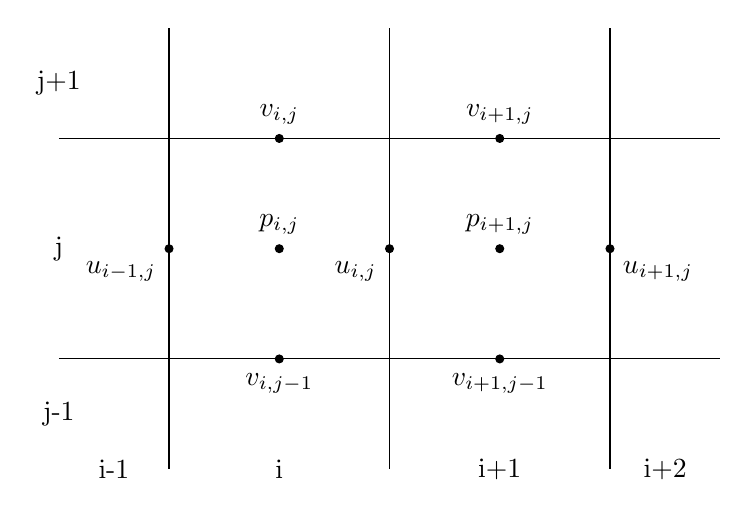
\begin{tikzpicture}[scale=1.4]

\draw (0, 1) -- (6, 1);
\draw (0, 3) -- (6, 3);

\draw (1,4) -- (1,0);
\draw (3,4) -- (3,0);
\draw (5,4) -- (5,0);

\node at (0, 0.5) {j-1}; 
\node at (0, 2) {j}; 
\node at (0, 3.5) {j+1};

\node at (0.5, 0) {i-1}; 
\node at (2, 0) {i}; 
\node at (4, 0) {i+1};
\node at (5.5, 0) {i+2};

\node[label=above:{$p_{i,j}$}, draw, circle, fill, minimum size=0.1cm, inner sep=0pt] at (2, 2) {};
\node[label=above:{$p_{i+1,j}$}, draw, circle, fill, minimum size=0.1cm, inner sep=0pt] at (4, 2) {};

\node[label=below left:{$u_{i-1,j}$}, draw, circle, fill, minimum size=0.1cm, inner sep=0pt] at (1, 2) {};
\node[label=below left:{$u_{i,j}$}, draw, circle, fill, minimum size=0.1cm, inner sep=0pt] at (3, 2) {};
\node[label=below right:{$u_{i+1,j}$}, draw, circle, fill, minimum size=0.1cm, inner sep=0pt] at (5, 2) {};

\node[label=above:{$v_{i,j}$}, draw, circle, fill, minimum size=0.1cm, inner sep=0pt] at (2, 3) {};
\node[label=above:{$v_{i+1,j}$}, draw, circle, fill, minimum size=0.1cm, inner sep=0pt] at (4, 3) {};

\node[label=below:{$v_{i,j-1}$}, draw, circle, fill, minimum size=0.1cm, inner sep=0pt] at (2, 1) {};
\node[label=below:{$v_{i+1,j-1}$}, draw, circle, fill, minimum size=0.1cm, inner sep=0pt] at (4, 1) {};

\end{tikzpicture}
    \caption{Discretization points for each variable on the staggered grid\cite{book:griebel1998numerical}}
    \label{fig:staggered_grid}
\end{figure}

Each of the variables is located at a different position on the grid cell.
Horizontal velocity $u_{i,j}$ is at the midpoint of the right cell edge, vertical velocity $v_{i,j}$ is at the midpoint of the top cell edge, and pressure $p_{i,j}$ is at the midpoint of the cell.
% Staggering the variables in this manner avoids oscillation in the pressure value caused by odd-even decoupling.
This is used to solve odd-even decoupling\cite{Harlow1965NumericalSurface}: for a fluid at rest (i.e. $u = v = 0$) the continuous solution is that the pressure $p$ is a constant across the grid.
However were this to be discretized using central differences with all variables in the same locations, it would also be possible for a checkerboard of pressure values to form, and for oscillation to take place\cite{book:griebel1998numerical}.
This is prevented by staggering the variables.
\cite{peric1988comparison} shows that this is also preventable through colocated grids, where a single grid is used for all variables and the velocities of each side of the cell are found using interpolation.
These cell sides are implicitly staggered relative to the pressure and so avoid this problem.

To allow for derivatives to be accurately calculated for cells on the edges of the grid, boundary cells are added around each grid.%\todomark{figure}
The cells on the edges of any obstacles in the simulation are also marked as boundary squares.
For a finite domain of size $(imax, jmax)$ this leads to a final grid size of $(imax + 2)$ by $(jmax + 2)$, where valid fluid values fall in the ranges %
%$1 \leq i \leq imax$, $1 \leq j \leq jmax$
$i \in \{1..imax\}$, $j \in \{1..jmax\}$.

The physical dimensions of each grid space are represented by \deltaX{}, \deltaY{}.
This allows the derivatives of $u$ and $v$ to be calculated by finding the centered differences.
\begin{align}
    \left[\frac{\partial{u}}{\partial{x}}\right]_{i,j} := \frac{u_{i,j}-u_{i-1,j}}{\delta{x}}, 
    & \quad %
    \left[\frac{\partial{v}}{\partial{y}}\right]_{i,j} := \frac{v_{i,j}-v_{i,j-1}}{\delta{y}}
\end{align}
% TODO multicolumn
% \begin{multicols}{2}
%   \begin{equation}
%     a=b
%   \end{equation}\break
%   \begin{equation}
%     b=c
%   \end{equation}
% \end{multicols}
The partial derivatives for pressure $\partial{p}/\partial{x}, \partial{p}/\partial{y}$ are found in the same way.
The remaining derivatives, including second derivatives and $\partial{uv}/\partial{x}, \partial{uv}/\partial{y}$, can also be discretized by taking the difference across midpoints of their respective dimensions\cite{hirt1976}.
%

\subsection{Simulation Stages}
\begin{figure}
    \centering

    \begin{tikzpicture}[
    scale=0.8, every node/.style={scale=0.8},
    stage/.style={minimum height = 2.5em, draw, anchor=north}
    ]
        \newcommand{\stagesep}{-0.4};
        \node[stage](s1) at (0,0) {Compute $\delta{t}$};
        \node[stage](s2) at ($(s1.south) + (0,\stagesep)$) {Compute Tentative Velocity};
        \node[stage](s3) at ($(s2.south) + (0,\stagesep)$) {Compute Poisson RHS};
        \node[stage](s4) at ($(s3.south) + (0,\stagesep)$) {Poisson Solver};
        % \node[stage](s5) at ($(s4.south) + (0,-0.6)$) {Poisson Iteration \#2};
        % \node[stage](s6) at ($(s5.south) + (0,-0.6)$) {...};
        % \node[stage](s7) at ($(s6.south) + (0,-0.6)$) {Poisson Iteration \#N};
        \node[stage](s8) at ($(s4.south) + (0,\stagesep)$) {Update Velocity};
        \node[stage](s9) at ($(s8.south) + (0,\stagesep)$) {Boundary Conditions};
    
        \draw[thick, ->] (s4.east) arc (0:-330:-0.4cm);% syntax (starting point coordinates) arc (starting angle:ending angle:radius)
        \node at ($(s4.east) + (2cm, 0)$){$N$ {}iterations}; 
    
        \draw[-latex] (s1.south) -- (s2.north);
        \draw[-latex] (s2.south) -- (s3.north);
        \draw[-latex] (s3.south) -- (s4.north);
        \draw[-latex] (s4.south) -- (s8.north);
        % \draw[-latex] (s5.south) -- (s6.north);
        % \draw[-latex] (s6.south) -- (s7.north);
        % \draw[-latex] (s7.south) -- (s8.north);
        \draw[-latex] (s8.south) -- (s9.north);
    \end{tikzpicture}
    \caption{Stages of a Simulation Tick}
    \label{fig:SimStages}
\end{figure}
Each simulation tick can be split into multiple stages, shown in \cref{fig:SimStages}.
These stages are described in detail in the following sections.

\subsection{Timestep Calculation}
\label{sec:TimestepCalculation}
Each simulation tick simulates a discrete amount of time known as a timestep \deltaT{}.
This timestep is not a fixed value, and typically one would want to select as large a timestep as possible.
However, there are constraints on it's maximum value which depend on the simulation state.

As the derivatives are calculated between adjacent grid points, it is impossible to accurately simulate a timestep where fluid moves between non-adjacent grid cells \todoref{Figure?}.
%[Peyret&Taylor,1983]or[Roache,1976].Anadaptivestepsizecontrolbasedonthesestabilityconditionsis usedin[Tome&McKee,1994].
% The simulation cannot accurately solve a timestep in which particles move completely over a cell (see Figure \todocite{}).
To prevent this the timestep \deltaT{} is calculated from the fluid velocities to make it impossible.
\begin{equation}
    \delta{t} = \tau * \text{min}\left(
        \frac{Re}{2}\left(
            \frac{1}{\delta{x}^2} + \frac{1}{\delta{y}^2}
        \right)^{-1},
        \frac{\delta{x}}{|u_{max}|},
        \frac{\delta{y}}{|v_{max}|}
    \right)
\end{equation}

Because the new velocities calculated in this tick may be larger than $u_{max}$ and $v_{max}$, the safety factor $\tau \in [0, 1]$ is used to ensure the timestep is large enough to account for it\cite{TOME1994171}.

\subsection{Tentative Velocity}
The final values of $u$ and $v$ are defined as
\begin{equation}
\begin{aligned}
    u^{(n+1)} &= u^{(n)} + \delta{t}
    \left[
        \frac{1}{Re}
        \paren{\partialderiv{^2u}{x^2} + \partialderiv{^2u}{y^2}} - \partialderiv{(u^2)}{x} - \partialderiv{(uv)}{y} + g_x - \partialderiv{p}{x}
    \right] \\
    v^{(n+1)} &= v^{(n)} + \delta{t}
    \left[
        \frac{1}{Re}
        \paren{\partialderiv{^2v}{x^2} + \partialderiv{^2v}{y^2}} - \partialderiv{(uv)}{x} - \partialderiv{(v^2)}{y} + g_y - \partialderiv{p}{y}
    \right]
\end{aligned}
\end{equation}
However, as these depend on the partial derivatives of $p$, which itself depends on velocity, they cannot be solved analytically.
In order to iteratively find $p$ the variables $f$ and $g$, for horizontal and vertical ``tentative velocity'', are introduced.
\begin{equation}
\begin{aligned}
    f^{(n)} := u^{(n)} + \delta{t}
    \left[
        \frac{1}{Re}
        \paren{\partialderiv{^2u}{x^2} + \partialderiv{^2u}{y^2}} - \partialderiv{(u^2)}{x} - \partialderiv{(uv)}{y} + g_x
    \right] \\
    g^{(n)} := v^{(n)} + \delta{t}
    \left[
        \frac{1}{Re}
        \paren{\partialderiv{^2v}{x^2} + \partialderiv{^2v}{y^2}} - \partialderiv{(uv)}{x} - \partialderiv{(v^2)}{y} + g_y
    \right]
\end{aligned}
\end{equation}
\begin{equation}
\begin{aligned}
    u^{(n+1)} = f^{(n)} - \delta{t}\frac{\partial{p^{(n+1)}}}{\partial{x}} \\
    v^{(n+1)} = g^{(n)} - \delta{t}\frac{\partial{p^{(n+1)}}}{\partial{y}}
    \label{eq:uv_modified}
\end{aligned}
\end{equation}

\subsection{Solving the Poisson Equation with SOR}
\label{sec:SimulationPoisson}
% Two phases - calculating the RHS, then solving
For continuity to be achieved, the final velocity values must fulfil the continuity equation (\cref{eq:NavierStokesContinuity}), the time discretization of which is shown below:
\begin{equation}
    \frac{\partial{u^{(n+1)}}}{\partial{x}} + \frac{\partial{v^{(n+1)}}}{\partial{y}} = 0
\end{equation}
This means that the total amount of fluid entering a cell in tick $n+1$ is equal to the amount of fluid leaving, which must be the case otherwise the amount of fluid per cell wouldn't be constant and the fluid would be compressed.

Substituting the formulae in \cref{eq:uv_modified} into this relation and rearranging gives
\begin{equation}
    \frac{\partial^2{p^{(n+1)}}}{\partial{x^2}} + \frac{\partial^2{p^{(n+1)}}}{\partial{y^2}} = \frac{1}{\delta{t}}\left(\frac{\partial{f^{(n)}_{i,j}}}{\partial{x}} + \frac{\partial{g^{(n)}_{i,j}}}{\partial{y}}\right)
\end{equation}
The right hand side of this equation is constant for timestep $n$, so can be precalculated and assigned to its own variable $rhs$.
\begin{equation}
rhs_{i,j} := \frac{1}{\delta{t}}\left(\frac{\partial{f^{(n)}_{i,j}}}{\partial{x}} + \frac{\partial{g^{(n)}_{i,j}}}{\partial{y}}\right)
\end{equation}
\begin{equation}
\frac{\partial^2{p^{(n+1)}}}{\partial{x^2}} + \frac{\partial^2{p^{(n+1)}}}{\partial{y^2}} = rhs_{i,j}
\end{equation}
Discretizing this gives
\newcommand{\discretized}[4]{#1^{#2}_{#3,#4}}
\newcommand{\pdisc}[3]{\discretized{p}{(#1)}{#2}{#3}}
\newcommand{\fdisc}[3]{\discretized{f}{(#1)}{#2}{#3}}
\newcommand{\gdisc}[3]{\discretized{g}{(#1)}{#2}{#3}}
\newcommand{\ebounds}[1]{\discretized{\epsilon}{#1}{i}{j}}
\begin{multline}
    \frac{\pdisc{n+1}{i+1}{j} - 2\pdisc{n+1}{i}{j} + \pdisc{n+1}{i-1}{j}}
    {(\delta{x})^2} + 
    \frac{\pdisc{n+1}{i}{j+1} - 2\pdisc{n+1}{i}{j} + \pdisc{n+1}{i}{j-1}}
    {(\delta{y})^2}
    % = \frac{1}{\delta{t}}\paren{
    %     \frac{\fdisc{n}{i}{j} - \fdisc{n}{i-1}{j}}{\delta{x}} + 
    %     \frac{\gdisc{n}{i}{j} - \gdisc{n}{i}{j-1}}{\delta{y}}
    % }
    = rhs_{i,j}
\end{multline}
and taking the simplest boundary conditions\cite{book:griebel1998numerical}
\begin{align}
    p_{0,j} &= p_{1,j}, & p_{i_{max+1},j} &= p_{i_{max},j} & j \in \{1..j_{max}\} \\
    p_{i,0} &= p_{i,1}, & p_{i,j_{max+1}} &= p_{i,j_{max}} & i \in \{1..i_{max}\} \\
    f_{0,j} &= u_{0,j}, & f_{i_{max},j} &= u_{i_{max},j} & j \in \{1..j_{max}\} \\
    g_{i,0} &= v_{i,0}, & g_{i,j_{max}} &= v_{i,j_{max}} & i \in \{1..i_{max}\}
\end{align}
resolves the equation to:
\begin{multline}
    \frac{\ebounds{E}(\pdisc{n+1}{i+1}{j} - \pdisc{n+1}{i}{j}) - \ebounds{W}(\pdisc{n+1}{i}{j} - \pdisc{n+1}{i-1}{j})}
    {(\delta{x})^2} \\
    + \frac{\ebounds{N}(\pdisc{n+1}{i}{j+1} - \pdisc{n+1}{i}{j}) - \ebounds{S}(\pdisc{n+1}{i}{j} - \pdisc{n+1}{i}{j-1})}
    {(\delta{y})^2}\\
    % = \frac{1}{\delta{t}}\paren{
    %     \frac{\fdisc{n}{i}{j} - \fdisc{n}{i-1}{j}}{\delta{x}} + 
    %     \frac{\gdisc{n}{i}{j} - \gdisc{n}{i}{j-1}}{\delta{y}}
    % }
    = rhs_{i,j}
    \label{eq:poisson_pre_sor}
\end{multline}
where $\epsilon_{i,j}^{\{N,S,E,W\}}$ represents the boundary squares (shown here for North, but it extends to the other directions)
\begin{equation}
    \epsilon_{i,j}^{N} = \begin{cases}
        0 & \text{The square directly above $i,j$ is a boundary}\\
        1 & \text{The square directly above $i,j$ is \emph{not} a boundary}
   \end{cases}
\end{equation}


\begin{figure}[ht]
\centering
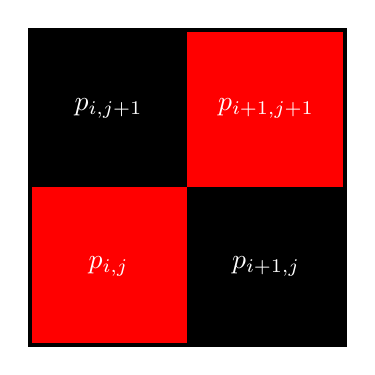
\begin{tikzpicture}[scale=1]
\draw[ultra thick, fill=red] (0,0) rectangle (4,-4);
    \foreach \row in {0,1} {
        \foreach \column in {0} {
    \fill ({4*\column + mod(\row,2)*2}, -\row*2) rectangle +(2,-2);
        }
    }
% \matrix (m) at (0,0) [matrix of nodes,nodes={},
%   anchor=north west,column sep={2cm,between origins},
%   row sep={2cm,between origins}] {
%  {\color{white}{$p_{i,j+1}$}} & {$p_{i+1,j+1}$} \\
%  {$p_{i,j}$} & {\color{white}{$p_{i+1,j}$}} \\
% };
\node at (1,-1) {\color{white}{$\bm{p_{i,j+1}}$}};
\node at (1,-3) {\color{white}{$\bm{p_{i,j}}$}};
\node at (3,-1) {\color{white}{$\bm{p_{i+1,j+1}}$}};
\node at (3,-3) {\color{white}{$\bm{p_{i+1,j}}$}};

% \matrix[matrix of nodes,nodes={draw}]{A & B & C & D & E\\f & G & H & I & J};
\end{tikzpicture}
    \caption{Example checkerboard pattern used for red/black splitting.}
    \label{fig:redblack_checkerboard}
\end{figure}
Over the whole grid, this results in a linear system of equations over the inputs $p_{i,j} \forall i \in \{1..i_{max}\}, j \in \{1..j_{max}\}$.
These can be decoupled by partitioning $p$ into red and black squares by a checkerboard pattern (see \cref{fig:redblack_checkerboard}).
As each individual cell only depends on the adjacent values, iterations of Successive Over-Relaxation (SOR) can be performed on red and black in turn to reach a final value\footnote{This could equally be done without partitioning $p$, but the partitioning splits the SOR into separate phases which can then be parallelized. Normal SOR cannot be parallelized\cite{Adams1982AMS}.}\cite{young1971iterative}:
\begin{equation}
    \beta_{i,j} := \frac{\omega}{\left(\frac{\epsilon_{i,j}^E+\epsilon_{i,j}^W}{(\delta{x})^2} + \frac{\epsilon_{i,j}^N+\epsilon_{i,j}^S}{(\delta{y})^2}\right)}
    \label{eq:poisson_beta}
\end{equation}
\begin{multline}
    p^{it+1}_{i,j} := (1 - \omega)p^{it}_{i,j} + \\
    \beta_{i,j} * \left(
    \frac{\epsilon_{i,j}^E p^{it}_{i+1,j}+\epsilon_{i,j}^W p^{it}_{i-1,j}}{(\delta{x})^2} + 
    \frac{\epsilon_{i,j}^N p^{it}_{i,j+1}+\epsilon_{i,j}^W p^{it}_{i,j-1}}{(\delta{y})^2} -
    rhs_{i,j}
    \right)
    \label{eq:poisson_final}
\end{multline}

These iterations are continued until the L2 norm\cite{l2norm} of the residuals (the difference between the left-hand side as calculated and the expected right-hand side of \cref{eq:poisson_final} for each cell) falls below a specific tolerance
% \footnote{In the ACA coursework this tolerance was relative to the L2 norm of $p$, although this was not directly specified by the book.}
\footnote{In the original simulation this tolerance was relative to the L2 norm of $p$, although this was not directly specified by the book.}
\cite{book:griebel1998numerical}.

\subsection{Final Velocity Calculations}
% Update Velocity, applyBoundaryConditions
Once the final values of $p$ have been calculated the velocity values $u,v$ can be found with \cref{eq:uv_modified}.
The boundary conditions for velocity must then be applied.
There are four relevant types of boundary condition\footnote{The book specifies five, including a Periodic Boundary Condition, which the original simulation did not support.}, which are applied depending on the type of boundary.
\begin{enumerate}
    \item No-Slip condition - no fluid penetrates the boundary, and fluid does not move past it i.e. the boundary applies friction.
    \item Free-Slip condition - fluid may not penetrate the boundary, but no friction is applied. Only tangential velocity is preserved for adjacent fluids.
    \item Inflow - fluid is flowing in constantly, so the velocity is set to a constant value. 
    \item Outflow - velocity perpendicular to the surface is preserved and fluids may flow out.
\end{enumerate}
% \todopending{Might need equations here?}

% \subsection{Overall Simulation Pipeline}


\section{Optimization}
\label{sec:Research:Optimization}
Optimizing simulations is important in all cases, even those that are not real-time, as it allows the engineers using the software to iterate faster on their designs.
When the extra constraint of real-time speeds is added, it becomes even more important.

\input{Ch20Research/Sub20_Opt_History}
\subsection{Previous Work}
\label{research:prev_work}
As work on CFD progressed some optimizations were developed that change the simulation pipeline and provide an overall speedup.
% Some of these were adapted into my ACA coursework submission\cite{modules:aca257submission}, which this project is based on, and carry over into the CUDA version.
Some of these were adapted into the original CPU simulation\cite{modules:aca257submission} and carry over into the CUDA version.
%, which this project is based on, and carry over into the CUDA version.


Given the definition of $\beta$ in \cref{eq:poisson_beta}, the value of $\beta_{i,j}$ does not change over the course of the simulation and so can be precalculated before the simulation starts.
Additionally, if it can be guaranteed that for every boundary square $p = 0$, which can be done either by never updating their pressure values or by updating them with $\beta_{i,j} = 0$, then $\epsilon_{i,j}$ doesn't need to be evaluated during the simulation at all.
These optimizations increased the runtime speed of the Poisson evaluation by 2.24x\footnote{The $\beta$ precalculation increased speed by 1.4x, and the removal of $\epsilon$ increased speed by 1.6x.\cite{modules:aca257submission}}, and they have been kept in the CUDA program.

The book states an alternate solution where $\epsilon$ is set to 1 at all times and pressure values on boundaries are copied from adjacent fluid squares\cite{book:griebel1998numerical}.
% This apparently stops noncontinuous starting velocities from producing nonphysical pressure values.
Using this method may prevent noncontinuous starting velocities from producing nonphysical pressure values.
Due to timing constraints this was not implemented for the simulation, but could be done in the future.
\label{ext:PressureValues}

% 1 on red/black
% The example implementation and the ACA implementation both use Red-Black Successive Over-Relaxation (SOR).
% Red-black SOR was first used to solve a system of linear equations on vector and parallel computersystems by Adams and Ortega [1], although introduced earlier (e.g., by Young [119]). Liu et al. [65] provideda more detailed analysis of red-black SOR implemented on GPUs
% NOTE - the Liu et al. there is a pretty close project

% In this method, the grid is split into red and black squares with a checkerboard pattern\todomark{figure}.
% First the values at red squares are updated, which depend only on the black squares.
% Then, the black squares are updated, which depend only on the red squares.
As stated in \cref{sec:SimulationPoisson}, red/black SOR is used to iteratively solve the Poisson equation.
% The red and black operations can be performed in parallel, but in both the ACA coursework and the CUDA program this has not been done\footnote{It has also been marked as a potential extension}.
% In the initial ACA coursework the values ($f$, $g$, $p$, $rhs$) for red and black data were stored in the same arrays.
In the initial CPU simulation the values ($f$, $g$, $p$, $rhs$) for red and black data were stored in the same arrays.
This was problematic as data of the same colour was never contiguous, and any iteration looking for just red values would get a cache line with both colours, leading to half of each cache line being wasted.
To fix this, red and black data is split into separate arrays before starting the Poisson solver.
This has been carried over into the CUDA implementation.

% Parallelization i.e. Vectorization, OpenMP?
% "The ACA coursework used OpenMP to provide thread-level parallelization in kernels, which is automatically provided when using a GPU."
The CPU simulation used OpenMP\cite{OpenMPHomeOpenMP} to automatically parallelize the Poisson solver (and other program elements) by column.
That is, each thread was given a group of columns to process.
This was not needed in the CUDA version as each GPU kernel is implicitly parallelized over many GPU threads.

The CPU simulation included optimizations exploiting properties of the original code, such as floating-point precision, to speed up calculations while producing identical results.
These optimizations include using fused multiply-add\cite{Muller2010TheInstruction} in some places (but not all), precalculating divisions with double-precision floats, and skipping the residual calculation phase altogether.
As this project was focused on improving upon the accuracy and speed of the original simulation, instead of producing bit-identical results, some of these optimizations were removed or made redundant.

% Paragraph on ACA-specific (FMA tricks, removing divisions, residual removal)
% "Other courseworks specifically tied to the ACA coursework were"...

%% ACA Recap(cite)
%% - Residual removal. (probably needs to be reversed)
%% - beta precalc (check if somewhere/ in book)
%% - mathematical optimization to remove branches (check if in book)
%% - FMA trickery (cite FMA properties)
%% - red/black rearranging (defo mentioned in top level paper, find citation from that)
%% - vectorization AVX/SSE (can most likely cite something here)
%%     - Note that 8-vector was tested,but 4-vector was faster
%% - removing divisions (maybe?)
%% - OpenMP (irrelevant here but can provide a citation? and should be noted because it provides parallelism which is then replaced by the GPU)


% TODO - tick pipeline figure with ACA additions (ex. r/b splitting)

\subsection{New Optimizations}
\label{sec:FutureOptimization}
CPUs and GPUs have very distinct designs, so when moving programs between them it's important to acknowledge optimization techniques that apply to one and not the other.
This section sums up the research into optimizing CUDA programs, which should be applied when designing/implementing the final program.

% CUDA devices are split into many threads, which are split into groups of 32 that are executed concurrently as a warp\cite{tool:CUDAProgrammingV1}.
CUDA devices combine groups of 32 threads into a `warp', and executes them concurrently\cite{tool:CUDAProgrammingV1}.
If the threads in a warp attempt to access multiple words in the same cache line, the access is \textit{coalesced}\cite{NVIDIAHowBlog} and only one cache line needs to be fetched for the warp to continue.
Otherwise if the accesses all touch different cache lines, every cache line needs to be fetched before execution can continue for any of the threads.
This should be accounted for when structuring GPU work.

% Const Restrict Pointers for __ldg (https://dl.acm.org/doi/pdf/10.1145/3238147.3241533 tries to do this automatically and found a perf boost, can cite that or cite other papers on it).
% \todomark{This seems more like a statement of an optimization than a "Future Work".}
The CUDA C Programming Guide\cite{NVIDIAGlobalGuide} states that read-only memory can be read into a special data cache using the \texttt{\_\_ldg()} intrinsic.
The compiler may insert this automatically when it detects that data must be read-only.
The use of \texttt{const} and \texttt{\_\_restrict\_\_} qualifiers on pointers that are read-only is encouraged to make read-only data obvious.
In \cite{10.1145/3238147.3241533} it was found that introducing these qualifiers where possible led to large speedups in pointer heavy applications, and while our case may not use many pointers this should still be implemented wherever possible.

% GPU Vectorization (cite).
The ACA solution used Intel AVX and SSE instructions\cite{IntelCorporationIntroductionExtensions} to calculate four Poisson values at once\footnote{Vectors of eight were tried but were found to be slower than four.}.
In the Progress Report\todocite{progress report} it was asserted that CUDA cores could use SIMD on four-element floating-point vectors, and that this could be exploited similarly.
However, this is not the case.
The only SIMD instructions CUDA allows are for integer vectors of 2x16-bit or 4x8-bit\cite{NvidiaCUDASIMD}.%\todocite{\url{https://docs.nvidia.com/cuda/parallel-thread-execution/index.html\#data-movement-and-conversion-instructions-ld}}.
As the simulation operates on 32-bit signed floating point, these instructions are not suitable.

% Mention parallelization with OpenMP
% did already?

% Highly optimized reductions (cite).
Calculating the simulation timestep and calculating the residual for a Poisson iteration both require a reduction over large blocks of data.
Highly parallel GPU optimizations have already been studied extensively, so it is trivial to implement a fast generic reduction kernel.
In \cite{CUDAParallelReduction} seven kernels are described, in ascending order of speed, and this should be used as the basis for the implementation.

CUDA Graphs \cite{GrayCUDAGraph2019Blog} are a CUDA feature that reduces CPU overhead by invoking a large amount of GPU work all at once, rather than with individual invocations.
Running a CUDA graph will always use the same arguments as when initially recorded, so any work that depends on data that changes quickly (such as a timestep) would not be suitable.
Profiling should be used to determine when CUDA graphs are suitable, then applied only in these cases to avoid overcomplicating the program.

\section{Visualization}\label{sec:Research:Visualization}
% For the engineers and scientists developing simulations, it is important for a visualization to be completely accurate and show the data in as much detail as possible.
% However there are other groups that may not have as deep of an understanding, but whose actions and decisions should still be informed by the simulation results.
\todomark{Viz intro}



% To ensure the visualization has an equivalent workload to real-world programs, understanding the current state of the art visualization techniques are 

% This all needs to be updated.

\subsection{Background}

% \todomark{New viz research background ya dingus}

% Para on normal viz, explain that it's old as a concept

% Introduce in-situ visualization

One of the earliest CFD interactive visualizations was in 2002, which had a simulation running slower than real time on a separate computer to the real-time visualization\cite{paper:2002vis:10.5555/509740.509745}.
%\todocite{https://dl.acm.org/doi/10.5555/509740.509745}
Decoupling the simulation speed from the visualization speed allowed for high framerates to be achieved for the user interface, however any changes made from the user interface had a delay of 0.5 seconds before being reflected in the simulation.
This qualifies as a loosely-coupled in-situ visualization, because simulation data is streamed to a separate visualization system while the simulation completes.

% Introduce current industrial tools (autodesk CFD, VTK)
A significant open-source toolkit is VTK\cite{VTKWebpage}, first introduced in 1993\cite{VTKBook}, which powers multiple tools such as ParaView\cite{ParaViewWebpage} and VisIt\cite{VisItWebpage}.
Both of these programs support tightly-coupled in-situ visualization of an external simulation with plugins, but the VTK base is not well suited to in-situ integration\cite{kress2017situ}.

Autodesk CFD\cite{AutodeskCFDWebpage} is a closed-source tool which integrates its own simulation and visualization together.
It's based on ALGOR FEA, created by ALGOR Inc which was acquired by Autodesk in 2008 \cite{AutodeskAcquiresALGOR}.
The latest iteration is targeted at the manufacturing industry, unlike VTK which is a generic toolkit, and does not support in-situ visualization.

Both of the above examples are not built for in-situ visualization, but these programs still represent the industry standard for visualization capabilities.
A novel element of this project is building a program from the ground up for in-situ visualization, and the visualization components will be based on Autodesk.
\subsection{Previous Work}\label{sec:Research:Viz:ACA}
The original simulation\cite{modules:CS257Coursework} included a simple image visualizer for a static state, which evaluated one of two quantities over the grid and produced a \shell{.ppm} image with the result.
These quantities were Vorticity ($\zeta$), the strength of vortical (a.k.a. rotational) motion at each point in the grid; and Stream Function ($\psi$), the contours of which define streamlines.
Streamlines are lines that are parallel to the velocity vector at each point, allowing the long-term flow of particles to be represented with a single line, and thus in a static image.\cite{NASADefinitionStreamlines}
The quantities are defined by \cref{eq:zeta,eq:vorticity}, as specified in \cite{book:griebel1998numerical}.
Examples of these modes are shown in \cref{fig:ppms}.

\begin{equation}
    \zeta(x,y) := \frac{\delta{u}}{\delta{y}} - \frac{\delta{v}}{\delta{x}}
    \label{eq:zeta}
\end{equation}
\begin{equation}
    \frac{\delta{\psi}(x,y)}{\delta{x}} := -v,\quad \frac{\delta{\psi}(x,y)}{\delta{y}} := u
    \label{eq:vorticity}
\end{equation}

\begin{figure}[ht]
    \centering
    \subcaptionbox{Vorticity $\zeta$\label{fig:zeta_ppm}%
    }[\linewidth]{\includegraphics[width=\linewidth,natwidth=660,natheight=120]{Ch20Research/figures/output_zeta.png}
    }
    
    \subcaptionbox{Stream Function $\psi$\label{fig:psi_ppm}%
    }[\linewidth]{\includegraphics[width=\linewidth,natwidth=660,natheight=120]{Ch20Research/figures/output_psi.png}
    }
    
    \subcaptionbox{Pressure $p$\label{fig:pressure_ppm}%
    }[\linewidth]{\includegraphics[width=\linewidth,natwidth=660,natheight=120]{Ch20Research/figures/output_pressure.png}
    }
    \caption{Examples of the three outputs available from the original visualization.}%\\These all visualize the output of a modified ACA coursework running for 10 seconds on the provided input data.
    %  all visualizing the same state.
    \label{fig:ppms}
\end{figure}
% Criticism of zeta, psi, pressure implementation
The vorticity image in \cref{fig:zeta_ppm} competently shows which areas of the grid contain particle movement.
Unfortunately, near the edges of the obstacle circle (shown in green) the edges are black, implying no movement or rotation, which is incorrect and also a distracting artefact for the viewer.
These are due to the imprecise nature of the original code, which only uses the differences to the East and South to find $\zeta$.
This breaks down when the squares in these directions are boundaries, and the program defaults to zero.
A better solution would be to take the central difference whenever possible and to fall back to using only one side when adjacent to a boundary.
This would mean the only points where this breaks down are where a square is surrounded by boundaries on opposite sides, which is much less likely and would also likely break other areas of the simulation.

The Stream Function visualization (\cref{fig:psi_ppm}) is nearly impossible to visually parse, which makes sense as the velocity information is encoded in the differences between adjacent squares and not directly in the colours.
The Stream Function is not intended to be directly visualized but instead used to find streamlines, which can be visualized directly.

\label{sec:VizPressureCritique}
During program development, a third mode was added which directly visualized the pressure values to aid in debugging, but this was not a very useful visualization as seen in \cref{fig:pressure_ppm}.
Pressure is only ever referenced in the Navier-Stokes equation (and subsequently the algorithm) as a relative value.
However, the simulation in practice ends up increasing all cells by a small amount each iteration.
This overall increase in pressure values is ignored by the simulation, but the visualization doesn't adjust for it.
In this example, the pressure values have all increased so even the lowest pressure value is a mid-grey.
If the program simulated for too long, the pressure values would become too high and the visualization would be entirely white.
This should be accounted for in the visualization, but also implies the base simulation is unstable.
The simulation stability will be touched on in Results/Evaluation (\cref{sec:Results,sec:Evaluation}).
\subsection{Current State-of-the-Art}
The nature of this project required the visualizations to be rebuilt from the ground up, both to work on the GPU correctly and to synchronize with the concurrent simulation.
This allowed new visualization features to be added.
As a starting point, the supported visualization features of Autodesk CFD 2019 were investigated, and are outlined in \cref{tab:AutodeskCFDSummary}.
This section will explain these features in more detail.

\begin{figure}[ht]
    \centering
    \includegraphics[width=\linewidth]{Ch20Research/figures/results_ribbon.png}
    \caption{Results Ribbon for Autodesk CFD 2019\cite[Results Visualization]{AutodeskCFDManual}}
    \label{fig:AutodeskCFDRibbon}
\end{figure}

\begin{table}[ht]
    \centering
    \begin{tabular}{c|c}
        Tool & Type \\
        \hline
        Global Controls & Visual \\
        Planes & Visual \\
        Iso Surfaces & Visual \\
        Iso Volumes & Visual \\
        Particle Traces & Visual \\
        \hline
        Wall Calculator & Text \\
        Parts & Text \\
        Points & Text \\
    \end{tabular}
    \caption{Summary of results tools from Autodesk CFD.}
    \label{tab:AutodeskCFDSummary}
\end{table}

Autodesk CFD is a 3D simulation/visualization, and typically involves placing one or more 3D surfaces (a 'model') and simulating the fluid movement around these surfaces.
The simulation process creates multiple quantities, including scalar quantities Speed, Temperature, Pressure; and Vector quantities such as Velocity.

\textbf{Global Controls}\cite[Global Controls]{AutodeskCFDManual} visualize selected quantities on all model surfaces.
A scalar quantity can be displayed by changing the surface color according to a scale (\cref{fig:AutodeskCFDGlobalControlsScalar}).
A vector quantity can be displayed by creating small arrows on the surfaces that represent the direction and magnitude of the quantity.
The range of displayed values can be changed for both the scalar and vector quantities.

A key limitation of this method is it does only shows the quantities on the surface, not the quantities inside the fluid.
Result Planes, Iso Surfaces, and Iso Volumes address this by calculating new surfaces/volumes which visualize quantities.
% These principles extend to most of the other visual tools, which generally define new surfaces to display quantities.

\begin{figure}
    \centering
    \includegraphics[width=\linewidth]{Ch20Research/figures/autodesk_cfd_global_results_scalar.PNG}
    \caption{Using the Global Controls to visualize a scalar result\cite{AutodeskCFDExercise7}}
    \label{fig:AutodeskCFDGlobalControlsScalar}
\end{figure}

\textbf{Results Planes}\cite[Planes]{AutodeskCFDManual} define a flat cross-section of the model which can visualize a single scalar quantity with a single vector quantity (\cref{fig:AutodeskCFDResultsPlane}).

\begin{figure}
    \centering
    \subcaptionbox{Scalar Quantity}[\linewidth]{\includegraphics[width=\linewidth]{Ch20Research/figures/autodesk_cfd_results_planes_scalar.png}}
    \subcaptionbox{Vector Quantity}[\linewidth]{\includegraphics[width=\linewidth]{Ch20Research/figures/autodesk_cfd_results_planes_vector.png}}
    \caption{Result Planes displaying different types of Quantity}
    \label{fig:AutodeskCFDResultsPlane}
\end{figure}

\textbf{Iso surfaces} define a surface based on the value of a result scalar quantity, e.g. $T = \SI{5}{\celsius}$.
This surface can then display a separate scalar and vector quantity, just like a Result Plane (\cref{fig:AutodeskCFDIsosurface}).

\begin{figure}
    \centering
    \includegraphics[width=\linewidth]{Ch20Research/figures/isosurface.png}
    \caption{An example of an Isosurface. ``The iso-surface shape indicates everywhere in the model that has a specific velocity magnitude. The colors indicate the static pressure at these locations.''}
    \label{fig:AutodeskCFDIsosurface}
\end{figure}

\textbf{Iso volumes} are similar to an isosurface, but define a volume based on a value range ($\SI{0}{\celsius} \leq T \leq \SI{5}{\celsius}$).
A vector quantity can be displayed at points within the volume, and the surface of the volume can show a scalar quantity.


\begin{figure}
    \centering
    \begin{subfigure}{0.45\textwidth}%
        \includegraphics[width=\linewidth]{Ch20Research/figures/autodesk_particle_comets.png}%
        \caption{Particle Comets}%
    \end{subfigure}%
    \begin{subfigure}{0.45\textwidth}%
        \includegraphics[width=\linewidth]{Ch20Research/figures/autodesk_particle_ribbons.png}%
        \caption{Particle Ribbons}%
    \end{subfigure}
    
    \begin{subfigure}{0.9\textwidth}%
        \includegraphics[width=\linewidth]{Ch20Research/figures/autodesk_particle_spheres.jpg}
        \caption{Particle Spheres}
    \end{subfigure}%
    \caption{Examples of Autodesk particle trails.}
    \label{fig:AutodeskCFDParticles}
\end{figure}

\textbf{Particle Traces} show the path particles would take through the flow after being emitted at certain points (or `seeds').
Autodesk allows these paths to be traced forwards or backwards, allows particles to be simulated both with mass and without, and allows a variety of particle trails to be shown (\cref{fig:AutodeskCFDParticles}).

\subsection{Stagnation \& Composition}
The techniques described above have been well known for at least 20 years.
The most prevalent algorithm for computing iso-surfaces was published in 1987\cite{LorensenMarching}.
% Source for marching-cubes being first? is https://www.routledge.com/Isosurfaces-Geometry-Topology-and-Algorithms/Wenger/p/book/9781466570979
Particle Traces and Results Planes were used in 1999\cite{Schulz1999}, although this is not the origin of either technique.
In some cases there has been extensive research into optimizing visualization techniques\cite{Ueng1996}, and in domain-specific areas there is academic research into creating new techniques\cite{Chen16}, but research into new generic visualization techniques has stagnated.
This stagnation was noted in \cite{vizRole2004} from 2004, which concluded the primary challenges facing visualization were ``identifying and characterizing features'' to visualize rather than developing new techniques.
The MET Office's weather reports demonstrate this principle, and show that composing multiple techniques together can increase information density while remaining easy to understand.

\begin{figure}
    \centering
    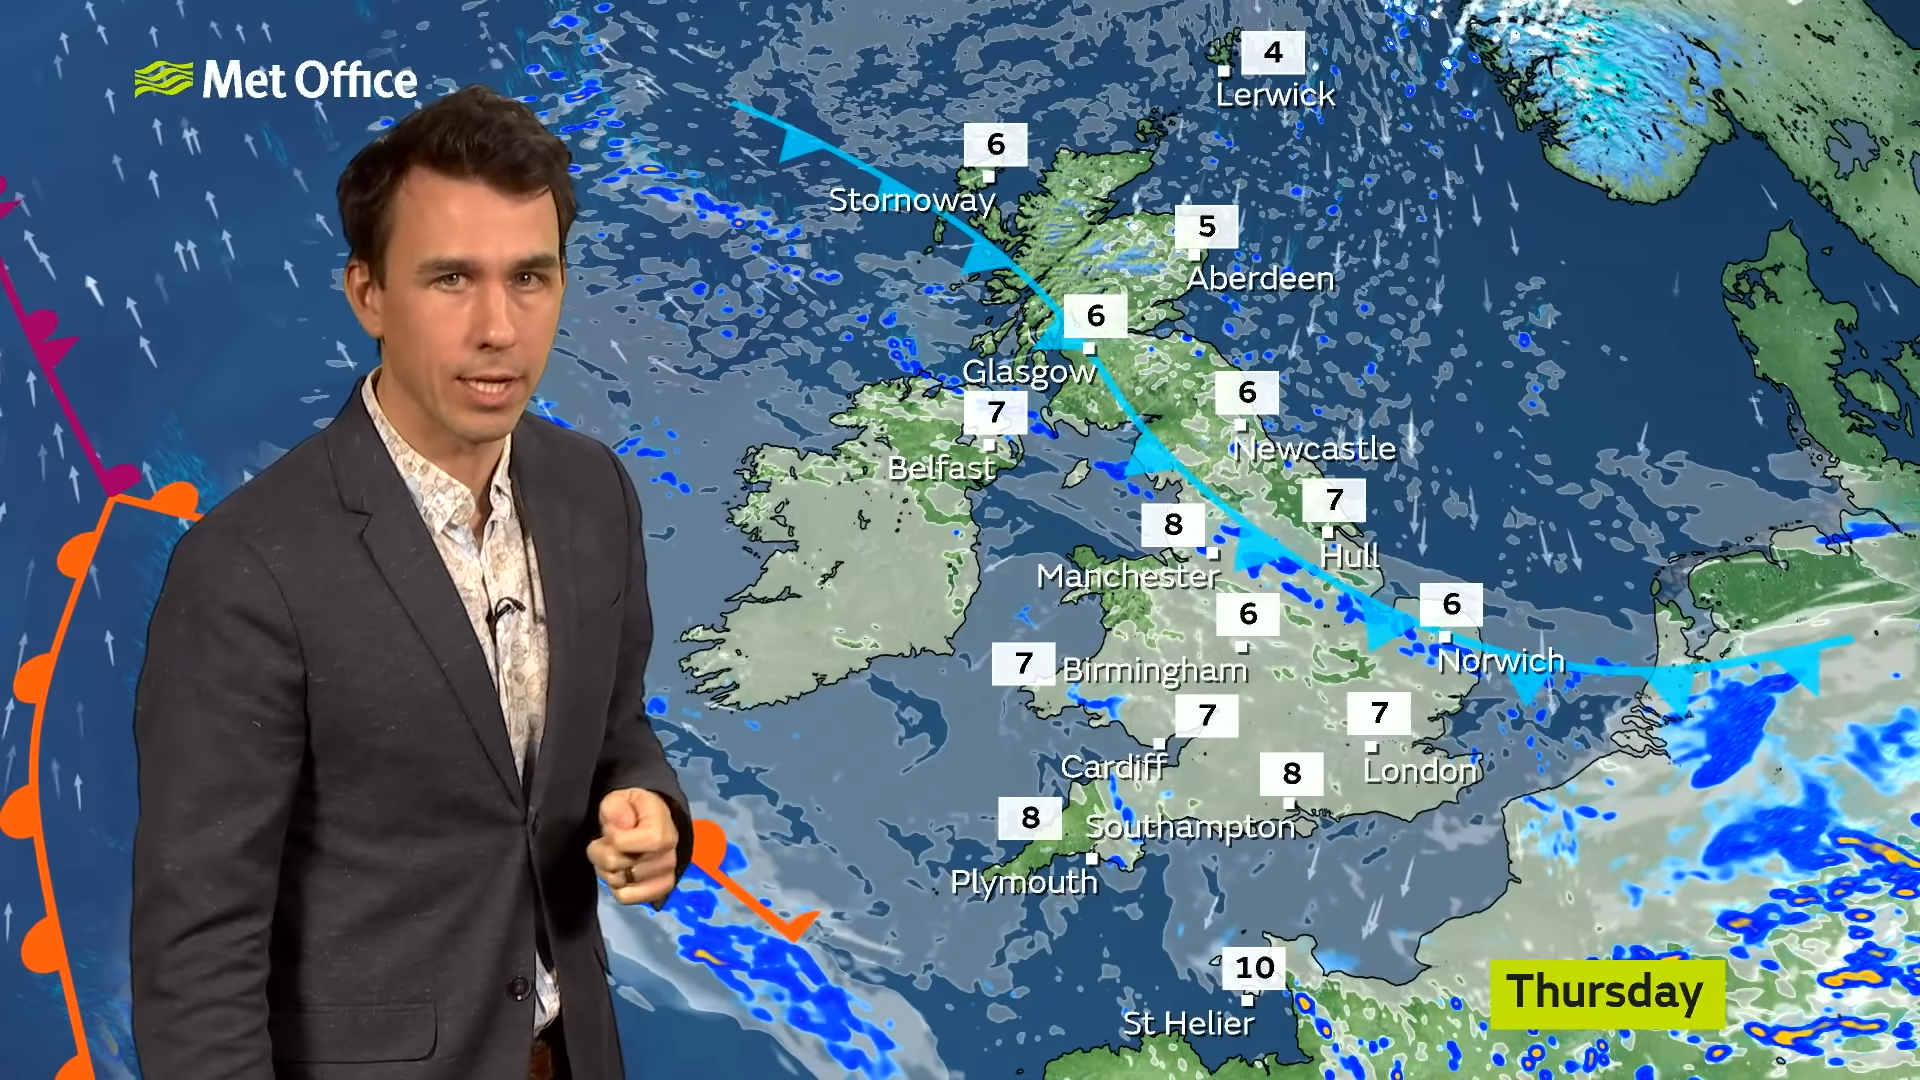
\includegraphics[width=\linewidth]{Ch20Research/figures/weather_better.PNG}
    \caption{MET Office weather report\cite{video:MetOfficeTenDayTrend}}
    \label{fig:MetOffice}
\end{figure}

\cref{fig:MetOffice} shows at least three visualization techniques used in the same image, each of which has been filtered to relevant points.
\begin{enumerate}
    \item The large blue, orange, and mauve lines show weather `fronts' moving in, the blue line particularly shows a cold front moving in from the north-east.
    \item The arrows show the wind direction, and only appear in areas with high wind speeds. In the video they also move, making it easier to understand at a glance.
    \item The gray and dark blue shape overlays show cloud cover and rain, respectively.
\end{enumerate}
This proves the potential of combining multiple techniques, which was taken into account when building the program.

\subsection{Realtime Particle Simulation Techniques}\label{sec:Research:Viz:Particles}
The particle simulation element of our visualization doesn't affect the simulation content, and does not have to be completely accurate as long as the flow is approximately correct for the viewer.
That is, the particle movement should fulfil \cref{eq:UnsteadyFlow}\cite{Lane93}
for the following variables:
\begin{itemize}
    \item $p = $ particle position.
    \item $t = $ time, and $t \in [t_1, t_n] \text{where} n = $ number of timesteps.
    \item $\vec{V}(p, t) = $ fluid velocity at point $p$ and time $t$.
\end{itemize}

\begin{figure}
\centering
\[ \frac{dp}{dt} = \vec{V}(p, t) \]

    \caption{Equation for particle movement in unsteady flow.}
    \label{eq:UnsteadyFlow}
\end{figure}
The unsteady-flow variant is shown because the fluid and particles will be moving at the same time, so the fluid itself is unsteady.

A common numerical method for accurately integrating this is the second-order Runge-Kutta scheme with adaptive timesteps, described in \cite{Lane93}.
This takes a constant step size $0 < c \leq 1$ which can be changed to control accuracy.
\begin{multline}
    h = c\norm{\vec{V}(p_k, t)}, \qquad p^{*} = p_k + h\vec{V}(p_k, t), \\
    p_{k+1} = p_k + h\frac{(\vec{V}(p_k, t) + \vec{V}(p^{*}, t + h))}{2}, \\
    t = t + h, \qquad k = k + 1
\end{multline}

A key issue with implementing this method in the program is that $\vec{V}$ is only kept in memory for one value of $t$, so interpolating between $\vec{V}(p_k, t) \text{and} \vec{V}(p^{*}, t + h)$ is impossible.
This also requires an indeterminate amount of steps, and potentially a different amount of steps for each particle, which is not GPU friendly.
Instead, a simpler version was chosen based on the steady-state variant.
At the instant the particle is simulated, the fluid is modelled as steady, and the particle moves with the same timestep taken by the simulation.
To avoid particles stepping over cells entirely, the timestep is subdivided into 4 iterations.

\begin{equation}
    \forall i \in [1..4] \qquad{} p_i = p_{i-1} + \vec{V}(p_{i-1}, t) / 4
\end{equation}
If $p$ does not align with a grid space, $\vec{V}(p)$ is trilinearly interpolated between the closest grid cells, as specified in \cite{Lane93}.

In addition to the particle simulation, particles must also be spawned and deleted when necessary.
GPU-based particle simulations are standard in video games, which need to run at high frame rates just like our visualization, so their techniques are a natural fit.
A notable method, which has been adapted for this program, is outlined in \cite{WickedEngineParticles}.
This splits the simulation into three phases:
\begin{enumerate}
    \item The kickoff phase, which determines the amount of new particles to create.
    \item The emission phase, which adds the required amount of new particles to the set by pulling from a queue of inactive particles.
    \item The simulation phase, which updates particle positions, adds dead particles to the inactive queue, and adds alive particles to a render queue.
\end{enumerate}


\subsection{Conclusions}
The research outlined so far has established common visualization methods, the potential for composing them together, and a design for an efficient particle simulation.
This was used to design the visualization (\cref{sec:Requirements}) and informed the implementation (\cref{fig:VizDataParticles}).